%%%%%%%%%%%%%%%%%%%%%%%%%%%%%%%%%%%%%%%%%%%%%%%%%%%
%% LaTeX book template                           %%
%% Author:  Amber Jain (http://amberj.devio.us/) %%
%% License: ISC license                          %%
%%%%%%%%%%%%%%%%%%%%%%%%%%%%%%%%%%%%%%%%%%%%%%%%%%%

\documentclass[a4paper,11pt]{report}
\usepackage[T1]{fontenc}
\usepackage[utf8]{inputenc}
\usepackage{lmodern}
%%%%%%%%%%%%%%%%%%%%%%%%%%%%%%%%%%%%%%%%%%%%%%%%%%%%%%%%%
% Source: http://en.wikibooks.org/wiki/LaTeX/Hyperlinks %
%%%%%%%%%%%%%%%%%%%%%%%%%%%%%%%%%%%%%%%%%%%%%%%%%%%%%%%%%
\usepackage{hyperref}
\usepackage{graphicx}
\usepackage[english]{babel}

\usepackage{listings}
\usepackage{xcolor}

\definecolor{codegreen}{rgb}{0,0.6,0}
\definecolor{codegray}{rgb}{0.5,0.5,0.5}
\definecolor{codepurple}{rgb}{0.58,0,0.82}
\definecolor{backcolour}{rgb}{0.95,0.95,0.92}

\lstdefinelanguage{JavaScript}{
	keywords={typeof, new, true, false, catch, function, return, null, catch, switch, var, if, in, while, do, else, case, break},
	keywordstyle=\color{blue}\bfseries,
	ndkeywords={class, export, boolean, throw, implements, import, this},
	ndkeywordstyle=\color{darkgray}\bfseries,
	identifierstyle=\color{black},
	sensitive=false,
	comment=[l]{//},
	morecomment=[s]{/*}{*/},
	commentstyle=\color{purple}\ttfamily,
	stringstyle=\color{red}\ttfamily,
	morestring=[b]',
	morestring=[b]"
}

\lstdefinestyle{mystyle}{
	backgroundcolor=\color{backcolour},   
	commentstyle=\color{codegreen},
	keywordstyle=\color{magenta},
	numberstyle=\tiny\color{codegray},
	stringstyle=\color{codepurple},
	basicstyle=\ttfamily\footnotesize,
	breakatwhitespace=false,         
	breaklines=true,                 
	captionpos=b,                    
	keepspaces=true,                 
	numbers=left,                    
	numbersep=5pt,                  
	showspaces=false,                
	showstringspaces=false,
	showtabs=false,                  
	tabsize=2,
	breaklines=true,
	postbreak=\mbox{\textcolor{red}{$\hookrightarrow$}\space}
}

\lstset{style=mystyle}

\graphicspath{ {../object_property_topic_maps/} }


%%%%%%%%%%%%%%%%%%%%%%%%%%%%%%%%%%%%%%%%%%%%%%%%
% Chapter quote at the start of chapter        %
% Source: http://tex.stackexchange.com/a/53380 %
%%%%%%%%%%%%%%%%%%%%%%%%%%%%%%%%%%%%%%%%%%%%%%%%
\makeatletter
\renewcommand{\@chapapp}{}% Not necessary...
\newenvironment{chapquote}[2][2em]
  {\setlength{\@tempdima}{#1}%
   \def\chapquote@author{#2}%
   \parshape 1 \@tempdima \dimexpr\textwidth-2\@tempdima\relax%
   \itshape}
  {\par\normalfont\hfill--\ \chapquote@author\hspace*{\@tempdima}\par\bigskip}
\makeatother

%%%%%%%%%%%%%%%%%%%%%%%%%%%%%%%%%%%%%%%%%%%%%%%%%%%
% First page of book which contains 'stuff' like: %
%  - Book title, subtitle                         %
%  - Book author name                             %
%%%%%%%%%%%%%%%%%%%%%%%%%%%%%%%%%%%%%%%%%%%%%%%%%%%

% Book's title and subtitle
\title{\Huge \textbf{CSE 6708 - Semantic Web} \\
	 \huge Techninal Documentation on Assignment 1 \\
	 \normalsize \textbf{Paper Name:} Source Code Plagiarism Detection Method Using Protégé Built Ontologies
}
% Author
\author{\textsc{Samidhya Sarker} \\ Student No. 1018052049 \\ Group-2}


\begin{document}

%\frontmatter
\maketitle

%%%%%%%%%%%%%%%%%%%%%%%%%%%%%%%%%%%%%%%%%%%%%%%%%%%%%%%%%%%%%%%%%%%%%%%%
% Auto-generated table of contents, list of figures and list of tables %
%%%%%%%%%%%%%%%%%%%%%%%%%%%%%%%%%%%%%%%%%%%%%%%%%%%%%%%%%%%%%%%%%%%%%%%%
\tableofcontents
\listoffigures
\lstlistoflistings
%\listoftables

%\mainmatter

%%%%%%%%%%%
% Preface %
%%%%%%%%%%%
\chapter{Introduction}
Software Plagiarism is defined as Copying Software without giving attribution. Ion Smeureanu and Bogdan Iancu
of the The Bucharest University of Economic Studies have written a scientific paper.
 In this paper, the authors devised a use of semantic web technologies to prevent software 


\section{Goals}
\begin{enumerate}
	\item Matching authors software implementation:
	\begin{itemize}
		\item Create ontologies from source code manually by hand using protege.
		\item Execute sparql queries on ontologies and compare the metrics.
		\item Create topic maps using Protege OntoGraf plugin.
	\end{itemize}
	\item Doing further works as dictated by the authors.
	\begin{itemize}
		\item Create a parser.
	\end{itemize} 
\end{enumerate}


\chapter{Emulating Experiments of Paper Authors}
\section{Creating ontologies}

\subsection{Tools Used}
	\begin{itemize}
		\item Protege 5.5.0 with OWL Code Generation Plug-in (2.0.0)
        \item VIM 8.1 with niklasl/vim-rdf and n3.vim Plug-in 
	\end{itemize}

\subsection{Source Code}
The authors of the paper had given two source codes in the paper that is identical in resulting output
but different lexically. The source code takes 3 numbers as input and outputs the maximum. \\

One is in the C programming language.
\lstinputlisting[language=C, caption=C source code for the max out of 3 program, label=c_source]{../src.c}
And another is in the Javascript programming language.
\lstinputlisting[language=JavaScript, caption=JavaScript source code for the max out of 3 program, label=js_source]{../src.js}

\subsection{Ontologies}
We convert the source code into schema ontologies by defining Classes, object properties, data properties
and individual code elements. The basic schema was given by authors and we extended it. 

We used RDF/XML OWL format for representing source ontologies because Protege is better suited for this than
RDF n3. it We get ontology \ref{c_owl}for the source code defined in \ref{c_source}.

We also got a OWL ontology \ref{js_owl} created from our javascript source code defined in \ref{js_source}

\section{SPARQL Query}
\subsection{Tools Used}
	\begin{itemize}
		\item Protege 5.5.0 with SPARQL Query Plug-in (3.0.0)
		\item VIM 8.1 with omer/vim-sparql Plug-In
	\end{itemize}
We used SPARQL Plug-In for Protege for executing sparql query in ontology \ref{c_owl} and \ref{js_owl}. Instead we could  have used Apache Jena Fuseki server \footnote{\url{https://jena.apache.org/}} for creating a SPARQL API endpoint.

We ran the following 8 SPARQL queries separately and got the expected results. 
\lstinputlisting[language=SPARQL, caption=SPARQL Queries given by the paper authors, label=sparql_source]{../query.sparql}

We matched the results given by the authors concluded the experiment as a success.

\section{Topic Maps}
\subsection{Tools Used}
\begin{itemize}
	\item Protege 5.5.0 with OntoGraf Plug-in (2.0.3)
\end{itemize}

For creating topic maps of the object properties of found ontologies, we used the OntoGraf Plug-In. We only showed 
the individual nodes not the class nodes and the properties associated with them as edges between nodes. We got the folling map of the C source ontology at \ref{c_owl} found from source \ref{c_source}. 

\begin{figure}[h]
	\label{c_ontology_topic_map}
	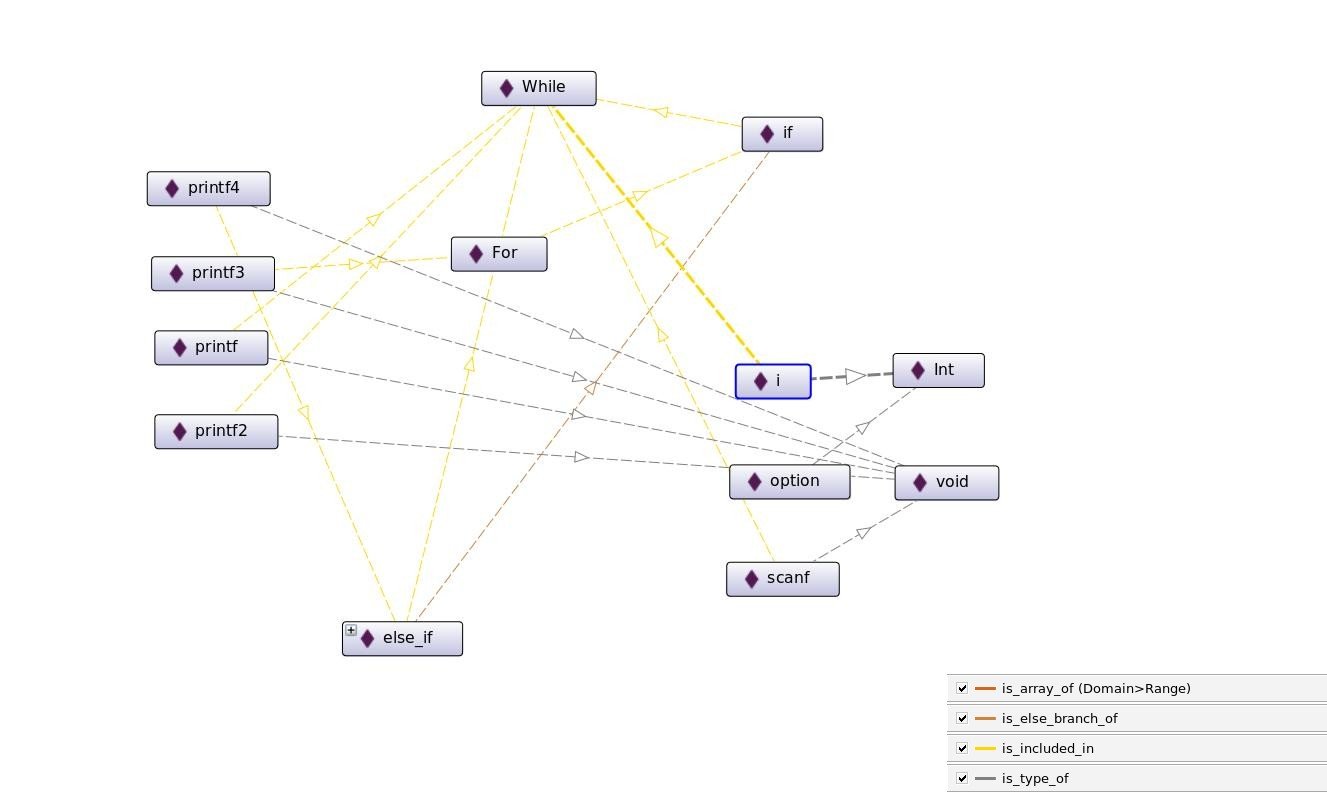
\includegraphics[scale=.35]{c_ontology_topic_map.jpg}
	\caption{Topic map ontology created by source code written in \ref{c_source} in C language}
\end{figure}

\break

In the same way we got the topic maps for the source \ref{js_source} for javascript language.

\begin{figure}[h]
	\label{js_ontology_topic_map}
	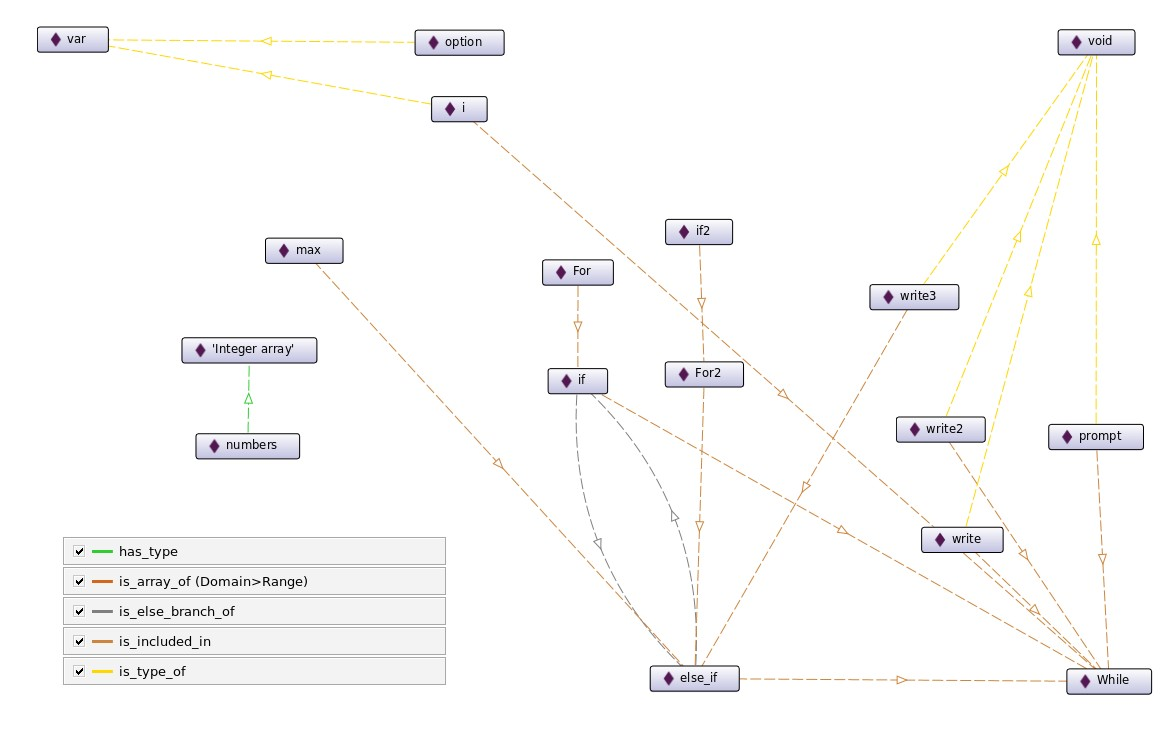
\includegraphics[scale=.35]{js_ontology_topic_map.jpg}
	\caption{Topic map ontology created by source code written in \ref{js_source} in JS}
\end{figure}

\break

\section{Conclusion}
Comparing the SPARQL query results and topic maps we can decide that the source code
of \ref{c_source} and \ref{js_source} has been plagiarized one from another.

\chapter{Implementation of specified further works of the paper}

In the further works section of the stated paper, the authors highlighted the following 
works that could be done:

\begin{enumerate}
    \item A parser for code.
    \item A crawler for parsing code.
    \item Dynamically generated SPARQL query for defined metrics.
\end{enumerate}

The creation of parser is the first step for the creation of an automated plagiarism detection system 
as envisioned by the authors. So, my research was focused on the formulation of a parser generator. 

\break

\section{An existing RDFized parser generator for the JAVA programming language: Codeontology}
The paper assigned to group-1 \footnote{CodeOntology: RDF-ization of Source Code} \footnote{\url{http://codeontology.org/}} already provides a RDF triple generating parser \footnote{\url{https://github.com/codeontology/parser}}. So for testing 
if it can cater to our needs, I transliterated out source \ref{c_source} and \ref{js_source} into Java programming language listed \ref{java_source}

\lstinputlisting[language=Java, caption=Java source code for the max out of 3 program, label=java_source]{../MaxOfThreeNumbers.java}

The main goal of the Codeontology project is to generate knowledge base for complex Java projects that
is different from our goal of detecting minute information of source codes. It does not take account of 
programming structures, only local variables, system functions and informations related to Java programming
environments like Package and Streams etc. This project can be modified to our liking and can also be adapted 
to other programming languages like C, Javascript. 

We get a highly complex topic map different that \ref{c_ontology_topic_map} and \ref{js_ontology_topic_map}.

\begin{figure}[h]
	\label{java_ontology_topic_map}
	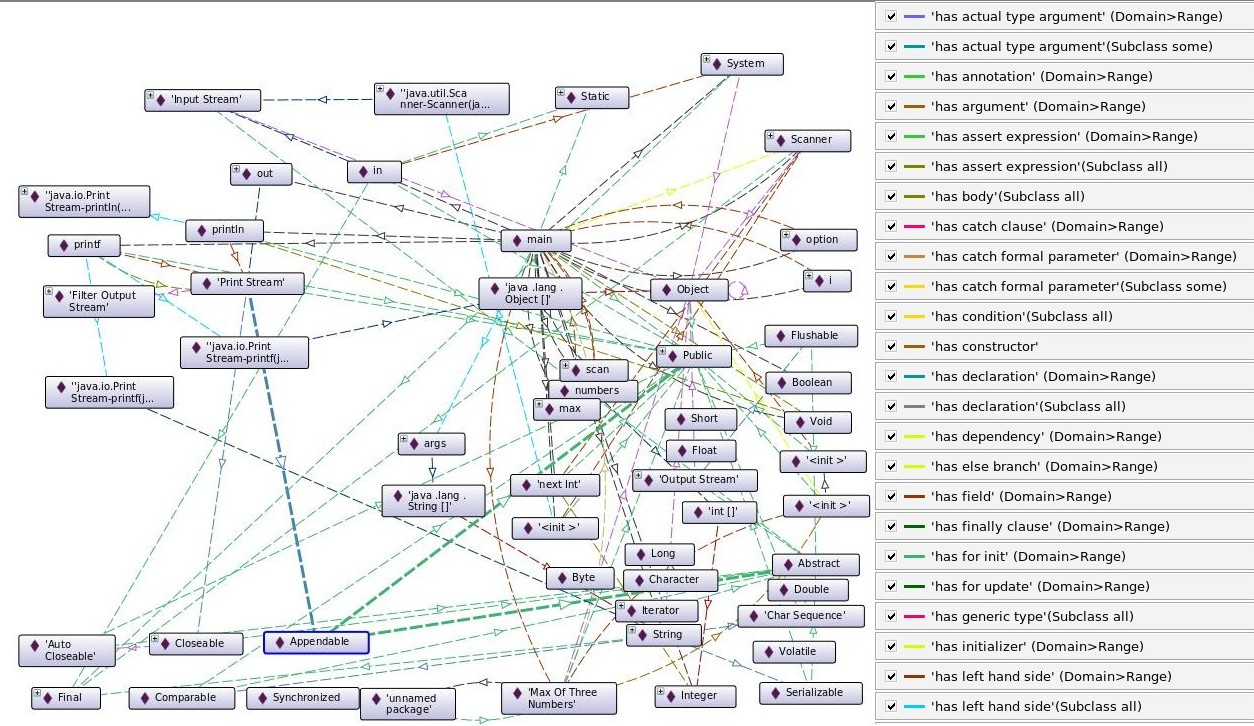
\includegraphics[scale=.35]{java_codeontology_topic_map.jpg}
	\caption{Topic map ontology created by source code written in \ref{java_source} in JAVA programming language}
\end{figure}

\section{Creating a Parser generator using ANTLR} \label{ANTLR}

ANTLR is a language recognition toolset which uses LL(*) grammer for parsing. There are language grammers available
including C \footnote{\url{https://github.com/antlr/grammars-v4/tree/master/c}}, JavaScript \footnote{\url{https://github.com/antlr/grammars-v4/tree/master/ecmascript}}, Java \footnote{\url{https://github.com/antlr/grammars-v4/tree/master/java}} etc. We used antlr to create a parse tree
for the C soruce described in \ref{c_source}

\begin{figure}
	\label{c_parse_tree}
	
\includegraphics[scale=.05]{antlr_parse_tree/c_antlr4_parse_tree.png}
	\caption{ANTLR parse tree created from C source at \ref{c_source}}
\end{figure}

Also, a parse tree for Javascript source from \ref{js_source} was also created.

\begin{figure}
	\label{js_parse_tree}
	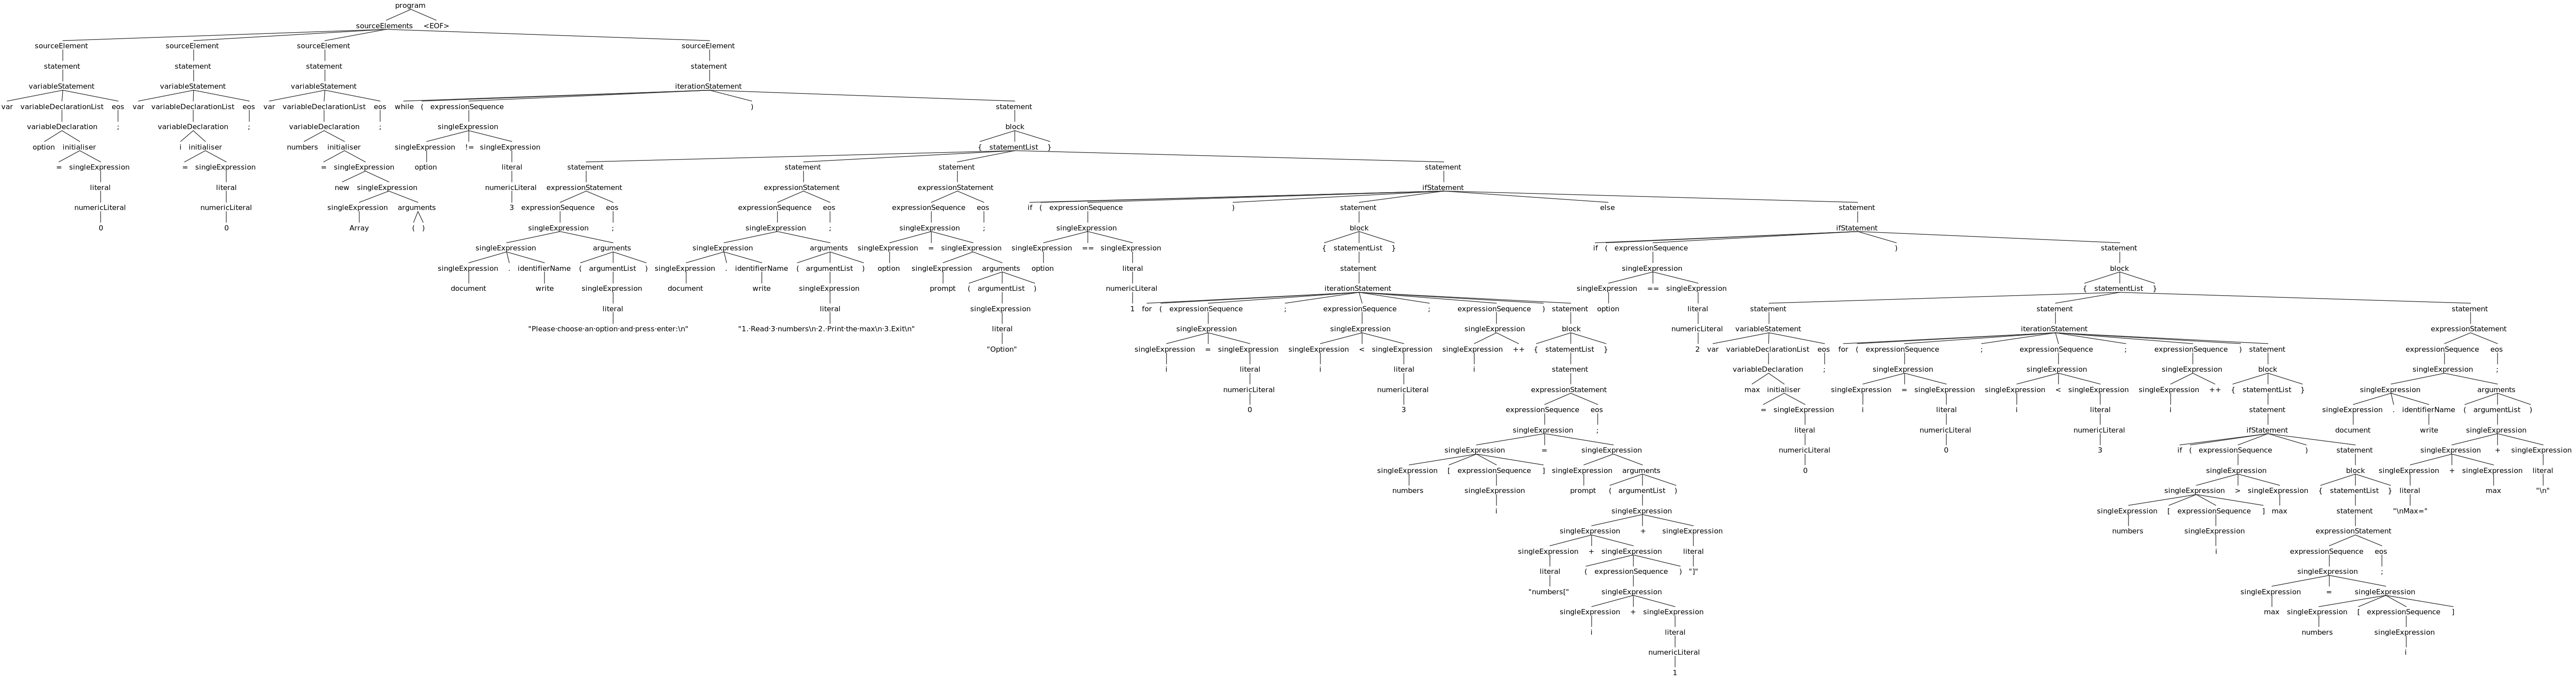
\includegraphics[scale=.08]{antlr_parse_tree/js_antlr4_parse_tree.png}
	\caption{ANTLR parse tree created from JS source at \ref{js_source}}
\end{figure}

So, ANTLR can certainly recognize C and JS source files. By modifying antler listener classes we can create 
toolset to generate dynamic rdf/xml files.

\section{Modifying Flex/Bison Code Generators to create RDF/XML generators} \label{FLEX_BISON}

Hypothetically, one can use the code generation techniques learned in CSE-310 course and modify the Assignment-4
(Code Generation) so that the parser generator outputs RDF/XML instead of ASSEMBLY code.

\footnote{\ref{ANTLR} and \ref{FLEX_BISON} has not been fully implemented due to time shortage.}

\chapter{Appendix}

\section{Owl soruce code for C source code defined in \ref{c_source}}
\lstinputlisting[language=xml, caption=Owl source code for C source code defined in \ref{c_source}, label=c_owl]{../c_source_ontology.owl}

\section{Owl soruce code for JavaScript source code defined in \ref{js_source}}
\lstinputlisting[language=xml, caption=Owl source code for JS source code defined in \ref{js_source}, label=js_owl]{../js_source_ontology.owl}

\end{document}
